\chapter{Методика исследования}

Как говорилось ранее, изучение параметров, характеризующих предварительное напряженное состояние грунта, чрезвычайно важно при инженерно-геологических изысканиях. В отечественной литературе и документах, долгое время этот факт оставался недооцененным. Соответственно, вопрос о значимости этих параметров оставался малоизученным до недавнего времени. Важно упомянуть, что в своей работе я только поверхностно исследую это проблему,  касаясь всего нескольких основных вопросов, связанных с компрессионными испытаниями, методами обработки полученных данных, а также их сравнением.

Представим историю существования некоторого сформировавшегося осадка. Коэффициент пористости, который характерен для данного осадка сразу после его формирования, называется седиментационным коэфициентом пористости. По мере увеличения толщи грунта, будет происходить его уплотнение, под действием напряжений от вышележащих слоев. Осадок будет уплотняться по линии <<нормального уплотнения>> или ветви первичной компрессии. В течение существования данного осадка возможна ситуация, когда напряжение будет снижаться, например, вследствие процесса выветривания, перемещения толщ грунта или появления и последующее исчезновения дополнительных нагрузок, создаваемых ледником. При этом будет наблюдаться некоторое разуплотнение осадка, однако оно не будет соответствовать ветви главного или первичного нагружения, потому что грунт является пластической средой  и большая часть накопленных деформаций является необратимыми. Точка при которой происхоит разгрузка называется точкой исторического давления. Если впоследствии нагрузка на данный грунт снова начнет увеличиваться, то сжатие будет происхоить по ветви повторного нагружения до тех пор, пока не дойдет до точки исторического давлении, а далее снова <<пойдет>> по главной ветви или по ветви первичного нагружения. Участок от точки начала повторного нагружения до точки пересечения с ветвью первичной компрессии не является прямой, из-за чего будет явное несоответствие между точкой начала рекомпрессии и точкой пересечения повторной нагрузки и ветви первичной компрессии. Это разница и привела к тому, что ученые всего мира начали искать методы, исключающие эту погрешность.

Одним из первых, кто ввел понятия <<нормально уплотненные грунты>> и <<переуплотненные грунты>> был австрийский и американский геолог Карл Терцаги. Под тезисом <<Нормально уплотненными грунтами>> Терцаги имел ввиду грунты, находящиеся под нагрузкой бытового давления. <<Переуплотненный>> же грунт, по его мнению, называется грунт, который при своем естесственном образовании находился под действием эффективных природных давлений, которые были больше, чем действующие в настоящее время бытовое давление. 


Корреляция двух графических методов фактически сводится к одному: их положительные и отрицательные стороны в разных компонентах. 

Если рассматривать с положительной точки зрения, то помимо простоты использования этих митодик также можно выделить и их удобство при обработке результатов испытаний, потому как метод позволяет фактически одним параметром  описать всю компрессионную кривую. Также, как преимущество у метода Беккера над методом Казагранде, можно считать тот факт, что тот посмтроен в линейном масштабе и не требует применения специального оборудования. В то же время в зависимости от типов грунтов, тот или иной метод может оказаться более чувствительнее, поэтому в ГОСТ 58326-2018 рекомендуется проводить обработку результатов всегда двумя способами и выбирать из них меньшее значение переуплотнения, то есть то, которое обеспечивает наибольший запас при проектировании.

 Метод, предложенный Артуром Казагранде хорошо зарекомендовал себя для глинистых грунтов, однако, графические методы несколько неудобны для инженерного использования, в нем присутствуют сложности, связанные с графическими построениями, в частности при получении длительных компрессионных кривых значительно усложняются условия решения задачи, потому как отсутствует участок кривой, где можно выделить видимое уплотнение грунта(точки максимальной кривизны графика с минимальным уклоном). Так же получаемые значения давления зависят от выбранного масштаба данного графика. Об этом же в своем исследовании и анализе говорил и известный бразильский ученый Пашеко Силва. Получаемое значение давления переуплотнения зависит от выбранного масштаба графика, что сильно влияет на полученные после обработки результаты.
 Зависимость от выбранного масштаба легко иллюстрируется на примере метода Пашеко Силва на рис 4.

 \begin{figure}
    \center{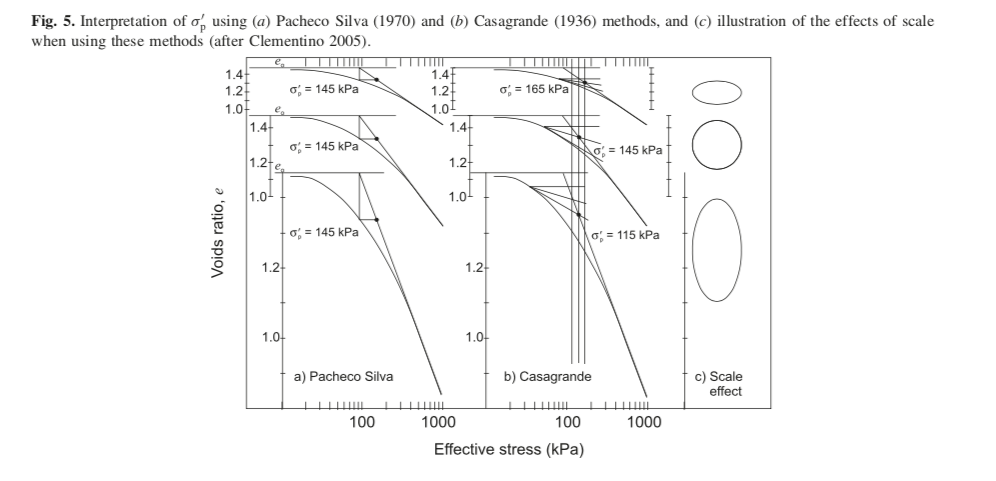
\includegraphics[scale=0.5]{3.png}
    \caption{рис.4 Сравнение методов Казагранде и Пашеко Силва.}
    \end{figure}
    
В свою очередь, методика Д.Беккера была применена к результатам, которые были получены после испытаний в одометре, на образцах глинистых грунтов природного сложения и на образцах с известным эффективным напряжением. Соотношение работы на единицу объема - эффективное напряжение. Оно может быть установлено с помощью линейных соотношений. Показано, что пересечение этих прямых, дает точные значения напряжений и предела текучести (предварительного уплотнения). Предел текучести определяется как пересечение исходной линии и линейной зависимости, наблюдаемой при более высоких напряжениях. На текущее эффективное напряжение указывает значительное расхождение данных с исходной установленной линией. Эти соотношения применимы как к условно горизонтально отобранным образцам, так и к вертикально отобранным образцам одометра. Выдвинута гипотеза, что действующие эффективные напряжения (как в вертикальном, так и в горизонтальном направлениях) в природной глине могут быть определены работой на единицу объема интерпретации компрессионных испытаний, проведенных на горизонтально и вертикально обрезанных образцах. ("критерии для определения природных и бытовых напряжений в глинах" D.Becker at all, 1987).

Беккер считает, что величина давления, равного суммарной работе, определяется давлением в конце приращения деформации. Полученная зависимость, как правило, имеет два прямолинейных участка. Напряжение, соответствующее точке пересечения двух прямых, проведенных к линейным участкам кривой, соответствует, по мнению Беккера, давлению предварительного уплотнения.
Соответственно, к недостаткам метода, так же как и для метода Казагранде, можно отнести наличие субъективного фактора при графических построениях, в частности сложность в выборе линейных участков, к которым проводятся прямые. 
